\documentclass[handout]{beamer}
\usepackage[dutch]{babel}
\usepackage{tikz,listings,multicol}
\usetikzlibrary{calc,shapes}
\usetheme{Antibes}
\setcounter{tocdepth}{2}
\title{Algoritmen en Gegevensstructuren 1:\\ \texttt{Array}, \texttt{ArrayList} en \texttt{LinkedList}}
\author{Willem Van Onsem\\ \href{mailto:vanonsem.willem@gmail.com?Subject=Presentatie\%20Algoritmen\%20en\%20Gegevensstructuren\%201}{vanonsem.willem@gmail.com}}
\AtBeginSection[]{\begin{frame}[plain]{Inhoud}
 \begin{multicols}{2}
 \tableofcontents[currentsection]
 \end{multicols}
\end{frame}}
\lstloadlanguages{Java}
\lstset{language=Java,basicstyle=\tiny\ttfamily}

\newcounter{tmpC}

\newcommand{\term}[1]{\textbf{#1}}

\newcommand{\dsarray}{\texttt{Array}}
\newcommand{\dsarraylist}{\texttt{ArrayList}}
\newcommand{\dslinkedlist}{\texttt{LinkedList}}
\newcommand{\dsint}{\texttt{int}}
\newcommand{\dsfloat}{\texttt{float}}
\newcommand{\dslong}{\texttt{long}}
\newcommand{\dsstring}{\texttt{String}}
\newcommand{\dsobject}{\texttt{Object}}

\newcommand{\tikzarray}[2]{
  \filldraw[fill=green!20,draw=black] (0,0) rectangle ++(#1*0.5,0.5);
  \foreach \x in {2,3,...,#1} {
    \draw (0.5*\x-0.5,0) -- ++(0,0.5);
  }
  \setcounter{tmpC}{0}
  \foreach \x in {#2} {
    \draw (0.25+0.5*\arabic{tmpC},0.25) node {\x};
    \addtocounter{tmpC}{1}
  }
}
\newcommand{\tikzarrayptr}[2]{
  \filldraw[fill=green!20,draw=black] (0,0) rectangle ++(#1*0.5,0.5);
  \foreach \x in {2,3,...,#1} {
    \draw (0.5*\x-0.5,0) -- ++(0,0.5);
  }
  \foreach \x in {1,2,...,#1} {
    \node[fill=black,circle,inner sep=0pt,minimum size=0.125cm] (#2\x) at (0.5*\x-0.25,0.25) {};
  }
}

\begin{document}
\begin{frame}[plain,fragile]
\maketitle
\end{frame}
\begin{frame}[plain]{Inhoud}
\begin{multicols}{2}
\tableofcontents
\end{multicols}
\end{frame}
\section{Array}
\subsection{Definitie}
\begin{frame}{Array: Definitie}
\begin{definition}[Array]
Een \term{\dsarray{}} is een gegevensstructuur die bestaat uit een opeenvolging van elementen. Elk element in een \dsarray{} heeft een unieke \term{index} en is toegankelijk in constante tijd (dit wordt ook wel \term{Random-Access} genoemd). Een \dsarray{} heeft een vaste \term{lengte} die bij de declaratie wordt toegekend. Eenmaal toegekend staat die lengte dus vast.
\end{definition}
%\begin{block}{Voorstelling}
Visueel zullen we een \dsarray{} in deze presentatie voorstellen als een opeenvolging van hokjes zoals hier:
\begin{figure}
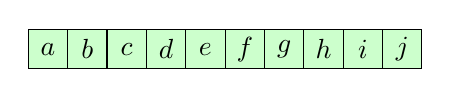
\begin{tikzpicture}
\filldraw[fill=green!20,draw=black] (0,0) rectangle (5,0.5);
\foreach \x in {1,2,...,9} {
  \draw (0.5*\x,0) -- ++(0,0.5);
}
\foreach \x/\t in {0/a,1/b,2/c,3/d,4/e,5/f,6/g,7/h,8/i,9/j} {
  \draw (0.5*\x+0.25,0.25) node {$\t$};
}
\end{tikzpicture}
\caption{Voorstelling van een \dsarray{}}
\end{figure}
%\end{block}
\end{frame}
\subsection{In Java}
\subsubsection{Declaratie}
\begin{frame}[fragile]{\dsarray{} in Java: declaratie}
In Java wordt een \dsarray{} aangemaakt door het type van de elementen te specificeren gevolgd door vierkante haken (\texttt{[]}). Tussen de vierkante haken wordt de lengte geplaatst:
\begin{example}[Declaratie \dsarray{}]
\begin{lstlisting}
int[] rijVanGetallen = new int[5];

int n = 20;
String[] rijVanStrings = new String[n];

int k = 5;
double[] rijVanDoubles = new double[n+k];
\end{lstlisting}
\end{example}
\end{frame}
\begin{frame}[fragile]{\dsarray{} in Java: declaratie: primitief versus klasse}
Java maakt een onderscheid tussen de declaratie van een array van \term{primitieve datatypes} (\dsint{}, \dsfloat{}, \dslong{},...) en \term{klasse-datatypes} (\dsobject{}, \dsstring{}):
\begin{enumerate}
 \item Bij primitieve datatypes wordt de \term{data} in de array opgeslagen.
 \begin{figure}[H]
 \centering
 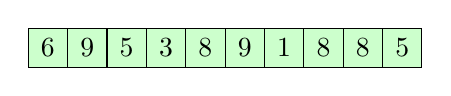
\begin{tikzpicture}
 \tikzarray{10}{6,9,5,3,8,9,1,8,8,5}
 \end{tikzpicture}
 \end{figure}
 \item Bij klasse-datatypes worden \term{pointers} in de array opgeslagen.
 \begin{figure}[H]
 \centering
 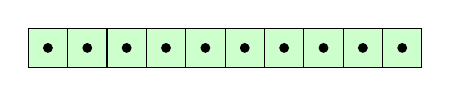
\begin{tikzpicture}
 \tikzarrayptr{10}{paex}
 \end{tikzpicture}
 \end{figure}
\end{enumerate}
\end{frame}
\subsubsection{Toegang tot elementen}
\begin{frame}[fragile]{\dsarray{} in Java: toegang tot elementen}
In Java kan men een element in een \dsarray{} opvragen door na de naam van de variabele tussen vierkante haken de index te vermelden. De index telt vanaf 0. Het eerste element staat dus op index 0. Men kan de waarde van een element in een array dan uitlezen en aanpassen.
\begin{example}[Toegang tot elementen van een \dsarray{}]
\begin{lstlisting}
int[] rijVanGetallen = new int[5];

rijVanGetallen[0] = 1;
rijVanGetallen[1] = 1;
rijVanGetallen[2] = rijVanGetallen[0]+1;
rijVanGetallen[3] = 5;
rijVanGetallen[4] = 8;
\end{lstlisting}
\end{example}
\end{frame}
\subsubsection{Lengte}
\begin{frame}[fragile]{\dsarray{} in Java: lengte}
In Java kan men de lengte van een \dsarray{} opvragen door het \texttt{length} argument op te roepen.
\begin{example}[Lengte opvragen van een \dsarray{}]
\begin{lstlisting}
int[] rijVanGetallen = new int[5];
System.out.println(rijVanGetallen.length);
\end{lstlisting}
\end{example}
\end{frame}
\section{ArrayList}
\subsection{Definitie}
\begin{frame}{\dsarraylist{}: definitie}
\begin{definition}[\dsarraylist{}]
Een \term{\dsarraylist{}} is een gegevensstructuur die bestaat uit een opeenvolging van elementen. Elk element in een \dsarraylist{} heeft een unieke \term{index} en is toegankelijk in constante tijd (dit wordt ook wel \term{Random-Access} genoemd). Een \dsarraylist{} heeft een variabele \term{lengte}: we hoeven geen lengte op te geven bij de constructie van een \dsarraylist{} en in principe kunnen we eindeloos elementen toevoegen.
\end{definition}
Visueel zullen we een \dsarraylist{} in deze presentatie voorstellen als een opeenvolging van hokjes, maar met een open einde. Zoals hier:
\begin{figure}
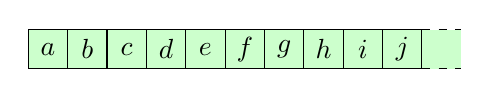
\begin{tikzpicture}
\fill[fill=green!20] (0,0) rectangle (5.5,0.5);
\draw (0,0) rectangle (5,0.5);
\draw[dashed] (5,0) -- ++(0.5,0);
\draw[dashed] (5,0.5) -- ++(0.5,0);
\foreach \x in {1,2,...,9} {
  \draw (0.5*\x,0) -- ++(0,0.5);
}
\foreach \x/\t in {0/a,1/b,2/c,3/d,4/e,5/f,6/g,7/h,8/i,9/j} {
  \draw (0.5*\x+0.25,0.25) node {$\t$};
}
\end{tikzpicture}
\caption{Voorstelling van een \dsarraylist{}}
\end{figure}
\end{frame}
\subsection{In Java}
\subsubsection{Declaratie}
\begin{frame}[fragile]{\dsarraylist{} in Java: declaratie}
Een \dsarraylist{} is een klasse die uit de Java-bibliotheek komt. Deze klasse is \texttt{java.util.ArrayList}. Daarom kunnen we een \dsarraylist{} aanmaken zoals andere objecten. Een \dsarraylist{} is een \term{generische klasse}: we kunnen een type-parameter tussen scheve haken (\texttt{<>}).
\begin{example}[Declaratie \dsarraylist{}]
\begin{lstlisting}
import java.util.ArrayList;

ArrayList<Integer> lijstMetGetallen = new ArrayList<Integer>();

ArrayList<Paard> lijstMetPaarden = new ArrayList<Paard>();

ArrayList<ArrayList<Integer>> lijstMetLijstenMetGetallen =
    new ArrayList<ArrayList<Integer>>();
\end{lstlisting}
\end{example}
\end{frame}
\subsubsection{Toegang tot elementen}
\begin{frame}{\dsarraylist{} in Java: toegang tot elementen}
Omdat \dsarraylist{} een gewone klasse is, krijgt met toegang tot de elementen via methodes:
\begin{itemize}
 \item \texttt{public E get (int index)}
 \item \texttt{public E set (int index, E element)}
\end{itemize}

\end{frame}
\subsubsection{Toevoegen en verwijderen}
\subsubsection{Andere operaties}
\subsection{Werking}
\subsection{Implementatie}
\section{LinkedList}
\subsection{Definitie}
\begin{frame}{\dslinkedlist{}: definitie}
\begin{definition}[\dslinkedlist{}]

\end{definition}
\end{frame}
\subsection{In Java}
\subsubsection{Declaratie}
\subsubsection{Toegang tot elementen}
\subsubsection{Toevoegen en verwijderen}
\subsubsection{Andere operaties}
\subsection{Werking}
\subsection{Implementatie}
\section{Interface}
\begin{frame}[fragile]{Interface}
\begin{definition}[Interface]
Een interface is een lijst van methodes die klasses die de interface implementeren moeten aanbieden.
\end{definition}
\begin{example}[\texttt{Praat}-interface]
\begin{lstlisting}
public interface Praat {

  void praat ();

}
\end{lstlisting}
\end{example}
\end{frame}
\subsection{Implementeren}
\begin{frame}[fragile]{Implementeren van een Interface}
Alle klasses die de interface \term{implementeren}, moeten de methodes invullen:
\begin{example}[Gert-klasse]
\begin{lstlisting}
public class Gert implements Praat {

  public void praat () {
    System.out.println("Hallo, mijn naam is Gert.");
  }

}
\end{lstlisting}
\end{example}
\begin{example}[Samson-klasse]
\small{\begin{lstlisting}
public class Samson implements Praat {

  public void praat () {
    System.out.println("Mwoa en ik ben Samson.");
  }

}
\end{lstlisting}}
\end{example}
\end{frame}
\end{document}
